\documentclass[a4paper,10pt]{article}
\setlength{\parindent}{0cm}
\usepackage{amsmath, amssymb, amsthm, mathtools,pgfplots}
\usepackage{graphicx,caption}
\usepackage{verbatim}
\usepackage{venndiagram}
\usepackage[cm]{fullpage}
\usepackage{fancyhdr}
\usepackage{tikz}
\usepackage{listings}
\usepackage{multirow,array}
\usepackage{color,enumerate,framed}
\usepackage{color,hyperref}
\definecolor{darkblue}{rgb}{0.0,0.0,0.5}
\hypersetup{colorlinks,breaklinks,
            linkcolor=darkblue,urlcolor=darkblue,
            anchorcolor=darkblue,citecolor=darkblue}
\usetikzlibrary{calc,matrix,positioning}
\pgfplotsset{compat=1.12}
%\usepackage{tgadventor}
%\usepackage[nohug]{diagrams}
\usepackage[T1]{fontenc}
%\usepackage{helvet}
%\renewcommand{\familydefault}{\sfdefault}
%\usepackage{parskip}
%\usepackage{picins} %for \parpic.
%\newtheorem*{notation}{Notation}
%\newtheorem{example}{Example}[section]
%\newtheorem*{problem}{Problem}
\theoremstyle{definition}
%\newtheorem{theorem}{Theorem}
%\newtheorem*{solution}{Solution}
%\newtheorem*{definition}{Definition}
%\newtheorem{lemma}[theorem]{Lemma}
%\newtheorem{corollary}[theorem]{Corollary}
%\newtheorem{proposition}[theorem]{Proposition}
%\newtheorem*{remark}{Remark}
%\setcounter{section}{1}

\newtheorem{thm}{Theorem}[section]
\newtheorem{lemma}[thm]{Lemma}
\newtheorem{prop}[thm]{Proposition}
\newtheorem{cor}[thm]{Corollary}
\newtheorem{defn}[thm]{Definition}
\newtheorem*{examp}{Example}
\newtheorem{conj}[thm]{Conjecture}
\newtheorem{rmk}[thm]{Remark}
\newtheorem*{nte}{Note}
\newtheorem*{notat}{Notation}

%\diagramstyle[labelstyle=\scriptstyle]

\lstset{frame=tb,
  language=Oz,
  aboveskip=3mm,
  belowskip=3mm,
  showstringspaces=false,
  columns=flexible,
  basicstyle={\small\ttfamily},
  breaklines=true,
  breakatwhitespace=true,
  tabsize=3
}

\DeclareMathOperator*{\argmin}{argmin}
\DeclareMathOperator*{\argmax}{argmax}
\newcommand*{\argminl}{\argmin\limits}
\newcommand*{\argmaxl}{\argmax\limits}

\pagestyle{fancy}




\fancyhead{}
\renewcommand{\headrulewidth}{0pt}

\lfoot{\color{black!60}{\sffamily Zhangsheng Lai}}
\cfoot{\color{black!60}{\sffamily Last modified: \today}}
\rfoot{\textsc{\thepage}}



\begin{document}

\section{Algorithmic Game Theory}
\subsection{Nonatomic Selfish Routing}
A selfish game occurs in a multicommodity flow network or simply a network. A network is given by a directed graph $G=(V,E)$, with vertex set $V$ and directed edge set $E$, together with a set $(s_1,t_1,),\ldots, (s_k,t_k)$ of source-sink vertex pairs which are called commodities. The $s_i-t_i$ paths of a network are denoted by $\mathcal{P}_i$ and we only consider networks in which $\mathcal{P}_i \neq \varnothing$ for all $i$, and define $\mathcal{P} = \bigcup_{i=1}^{k}\mathcal{P}_i$. The graph $G$ is allowed to have parallel edges and a vertex can participate in multiple source-sink pairs. The routes chosen by players are described by using flows, which is a nonnegative vector indexed by the set $\mathcal{P}$ of source-sink paths.
\begin{defn}
For a flow $f$ and path $P \in \mathcal{P}_i$, $f_P$ is the amount of traffic of commodity $i$ that chooses the path $P$ to travel from $s_i$ to $t_i$. A flow is feasible for a vector $r$ if it routes all the traffic: for each $i\in \{1, 2, \ldots, k\}$, $\sum_{P\in \mathcal{P}_i}f_P=r_i$.
\end{defn}

For each edge $e$ of the network has a cost function $c_e: \mathbb{R}^+ \to \mathbb{R}^+$ with the assumptions that the $c_e$'s are nonnegative, continuous and nondecreasing. For any nonatomic selfish routing game, or simply a nonatomic instance, we define it by a triple of the form $(G,r,c)$.

\begin{defn}
The cost of a path $P$ with respect to the flow $f$ is defined as the sum of the costs of the constituent edges: $c_p(f)=\sum_{e\in P}c_e(f_e)$, where $f_e=\sum_{P\in \mathcal{P}_i:e \in P}f_P$ denotes the amount of traffic using the paths  that contain the edge $e$.
\end{defn}

\begin{defn}[Nonatomic equilibrium flow]
Let $f$ be a feasible flow for an nonatomic instance $(G,r,c)$. The flow $f$ is an \emph{equilibrium flow} if, for every commodity $i \in \{1,2, \ldots, k\}$ and every pair $P, \tilde{P} \in \mathcal{P}_i$ of $s_i-t_i$ paths with $f_P>0$, 
\begin{align*}
c_p(f) \leq c_{\tilde{P}}(f)
\end{align*}
\end{defn}

\begin{defn}
The social cost of a flow $f$ is
\begin{align*}
SC(f) = \sum_{P\in \mathcal{P}}c_P(f)f_P
\end{align*}
we can also rewrite it by summing up the cost over all the edges in the network and it turns out that this representation is a useful trick for some proofs.
\begin{align*}
SC(f) = \sum_{e\in E}c_e(f_e)f_e
\end{align*}
For any instance $(G,r,c)$, a feasible flow is called an \emph{optimal flow} if it minimizes the social cost over all feasible flows. 
\end{defn}

In examples later, we see that equilibrium flows have social cost higher than optimal flow and although the ideal scenario is for the network to achieve the optimal flow, due to the selfish nature, the network is running on the equilibrium flow. The measure we use to see how bad the equilibrium flow is compared to the optimal flow is the price of anarchy which is defined as follows.

\begin{defn}
The price of anarchy of a nonatomic selfish routing game is the ratio of the cost of an equilibrium flow and that of an optimal flow.
\end{defn}


\begin{thm}[Existence and uniqueness of equilibrium flows]
Let $(G,r,c)$ be a nonatomic instance.
\begin{enumerate}[(a)]
\item The instance $(G,r,c)$ admits at least one equilibrium flow.
\item If $f$ and $\tilde{f}$ are equilibrium flows for $(G,r,c)$, then $c_e(f_e)=c_e(\tilde{f}_e)$ for every edge $e$.
\end{enumerate}
\begin{proof}
to be done later
\end{proof}
\end{thm}

\begin{defn}
Let $c_e^\ast(x)=(x\cdot c_e(x))'$ denote the \emph{marginal cost function} for the edge $e$.
\end{defn}

\begin{prop}[Characterization of optimal flows]
Let $(G,r,c)$ be a nonatomic instance such that for every edge $e$, the function $x\cdot c_e(x)$ is convex and continuously differentiable. Let $c_e^\ast$ denote the marginal cost function of the edge $e$. Then $f^\ast$ is an optimal flow $(G,r,c)$ iff for every commodity $i\ in \{1,2,\ldots, k\}$ and every pair $P, \tilde{P} \in \mathcal{P}_i$ of $s_i-t_i$ paths with $f_p^\ast>0$
\begin{align*}
c_p^\ast(f^\ast) \leq c_{\tilde{p}}^\ast(f^\ast)
\end{align*}
\end{prop}

\begin{cor}[Equivalence of equilibrium and optimal flows]\label{cor:equiv}
Let $(G,r,c)$ be a nonatomic instance such that for every edge $e$, the function $x\cdot c_e(x)$ is convex and continuously differentiable. Let $c_e^\ast(x)$ denote the marginal cost function of the edge $e$. Then $f^\ast$ is an optimal flow for $(G,r,c)$ iff it is an equilibrium flow for $(G,r,c^\ast)$.
\end{cor}
The consequence above says that there is a one to one correspondence between an optimal flow for $(G,r,c)$ and the equilibrium flow for $(G,r,c^\ast)$. In real life scenarios, the equilibrium flow is easily achieved as every agent selfishly tries to maximize their utility or minimize their cost, but the optimal equilibrium is not so obvious as some agents might have to be ``sacrificed'' in order to get a minimal social cost. Therefore, to find the optimal flow for $(G,r,c)$, we could do it by finding the equilibrium flow of $(G,r,c^\ast)$



\begin{defn}[Pigou-like networks]
A Pigou-like network is one with the traffic being routed, $r>0$ and consists of two nodes and two links: one with cost function $c(x)$ and the other with a constant cost fixed at $c(r)$, i.e. cost function of the upper cost function $c(x)$ evaluated at $r$.
\end{defn}

\begin{figure}[h]
\centering
\def\layersep{2.5cm}
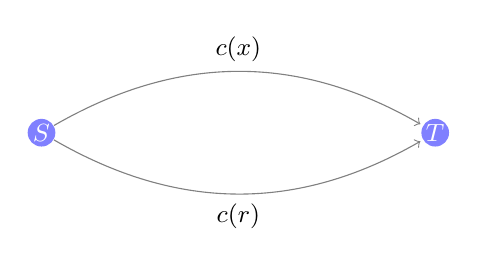
\begin{tikzpicture}[scale = 1,shorten >=1pt,->,draw=black!50, node distance=\layersep]
    \tikzstyle{every pin edge}=[<-,shorten <=1pt]
    \tikzstyle{neuron}=[circle,fill=black!25,minimum size=10pt,inner sep=0pt]
    \tikzstyle{output neuron}=[neuron, fill=red!50];
    \tikzstyle{n}=[neuron, fill=blue!50];

\node[n] (a) at (0,0) {\small\color{white}{$S$}};
\node[n] (b) at (5,0) {\small \color{white}{$T$}};
\draw (a) edge[bend right] node[below] {\small $c(r)$} (b);
\draw (a) edge[bend left] node[above] {\small$c(x)$} (b);
\end{tikzpicture}
\caption{Pigou-like network with traffic $r$}\label{fig:pigoulike}
\end{figure}
\begin{defn}[Pigou bound]
Let $\mathcal{C}$ be a nonempty set of cost functions. The \emph{Pigou bound} $\alpha(\mathcal{C})$ for $\mathcal{C}$ is 
\begin{align*}
\alpha(\mathcal{C}) = \sup_{c \in \mathcal{C}} \sup_{x,r\geq 0} \frac{r \cdot c(r)}{x\cdot c(x)+(r-x)c(r)}
\end{align*}
\end{defn}

\begin{thm}[Tightness of the Pigou bound]
Let $\mathcal{C}$ be the set of cost functions and $\alpha(\mathcal{C})$ the Pigou bound for $\mathcal{C}$. If $(G,r,c)$ is a nonatomic instance with cost functions in $\mathcal{C}$, then the price of anarchy of $(G,r,c)$ is at most $\alpha(\mathcal{C})$.
\begin{proof}
the idea is to instantiate each edge as a pigou-like network.
\end{proof}
\end{thm}



\subsection{Network Overprovisioning}
Let us now consider selfish routing networks with cost function
\begin{align*}
c_e(x):=\begin{cases}
\frac{1}{R_e-x} &\text{ if } x < R_e\\
+\infty & \text{ if }x \geq R_e
\end{cases}
\end{align*}
\begin{defn}
A network is $\beta-$overprovisioned, meaning
\begin{align*}
f_e\leq (1-\beta)R_e
\end{align*}
for all edges $e \in E$ at equilibrium where $R_e$ is the capacity of edge $e$.
\end{defn}
The worst case price of anarchy in $\beta-$overprovisioned networks is at most
\begin{align*}
PoA = \frac{1}{2}\left(1+\sqrt{\frac{1}{\beta}}\right)
\end{align*}
from the above result, we can observe that
\begin{alignat*}{2}
\beta &\to 1,\quad &PoA &\to 1\\
\beta &\to 0, \quad&PoA &\to \infty\\
\end{alignat*}
Recall that for nonlinear Pigou's example we have the price of anarchy to be unbounded. Hence to 

\begin{thm}
If $f$ is an equilibrium flow for $(G,r,c)$ and $f^\ast$ is a feasible for $(G,2r,c)$, then $SC(f)\leq SC(f^\ast)$.
\begin{proof}
By the definition of equilibrium flow, we have
\begin{align*}
\sum_{e\in E}c_e(f)f_e=\sum_{P\in\mathcal{P}}c_P(f)f_P = r\cdot L
\end{align*}
where $L$ is the common cost of every path the equilibrium flow. Fixing the cost of the paths at the equilibrium flow but changing the flow to the optimal flow instead, we get
\begin{align*}
\sum_{e\in E}c_e(f)f^\ast_e=\sum_{P\in\mathcal{P}}c_P(f)f_P^\ast \geq 2r\cdot L
\end{align*}
To complete the proof, it suffices to show that: 
\begin{align*}
\sum_{e\in E}c_e(f^\ast)f^\ast_e \geq \sum_{e\in E}c_e(f)f^\ast_e-\sum_{e\in E}c_e(f)f_e
\end{align*}
We will show the above by showing that for each edge $e\in E$
\begin{align*}
f_ec_e(f_e) \geq f_e^\ast(c_e(f_e)-c_e(f_e^\ast))
\end{align*}
which says that the error made in using the cost of the edges at the equilibrium flow instead of the optimal flow is at most the cost at the equilibrium flow. By considering cases:
\begin{enumerate}[(i)]
\item $f_e\leq f_e^\ast$ which will give a negative right term as $c_e$ is a nondecreasing function thus the inequality is clearly true.
\item $f_e > f_e^\ast$
add diagram here.
\end{enumerate}
\end{proof}
\end{thm}


\subsection{Location Games}


\subsection{Positive Externalities}
A \emph{network cost-sharing game} takes place in a graph $G=(V,E)$ which can be directed and undirected and each edge $E$ carries a fixed cost $\gamma_e\geq 0$. There are $k$ players and each player $i$ has a source vertex $s_i \in V$ and a sink vertex $t_i\in V$ and its strategy set is the $s_i-t_i$ paths of the graph. Outcomes of the game are path vectors $(P_1,\ldots,P_k)$, with the semantics that the subnetwork $(V,\cup_{i=1}^{k}P_i)$ gets formed. 

The $\gamma_e$ is thought of as a fixed cost for building edge $e$, i.e. laying down high-speed internet fiber to a neighbourhood and this cost is independent of the number of users using that edge. The cost incurred by a player is the sum of all the cost of the edges used by the player, but instead of incurring higher cost for a highly utilized edge, the cost is lower when more people are using that edge, hence its name. Let $\ell_e$ denote the load of an edge $e$ and for $\ell_e>0$, the players that utilize edge $e$ are jointly responsible for the fixed cost of the edge, $\gamma_e$. Here we will assume that the cost of an edge are split equally amongst the players. The cost of a player $i$ is thus given by
\begin{align*}
C_i(\mathbf{P})=\sum_{e\in P_i}\frac{\gamma_e}{\ell_e}
\end{align*}
where $\ell_e=|\{i:e \in P_i\}|$ is the number of players that chooses a path the includes $e$. Our objective is to minimize the total cost of the formed network
\begin{align*}
cost(\mathbf{P}=\sum_{e\in E:\ell_e>0}^{})
\end{align*}


%\begin{defn}
%For any finite game, an \emph{exact potential function} $\Phi$ is a function that maps every strategy vector $S$ to some real value and satisfies the following condition: If $S=(S_1,S_2, \ldots, S_k)$, $S'_i\neq S_i$ is an alternative strategy for some player $i$, and $S'=(S_{-i},S'_i)$, then
%\begin{align*}
%\Phi(S)-\Phi(S') = u_i(S)-u_i(S')
%\end{align*}
%\end{defn}

%\section{Algorithmic Game Theory}
%\subsection*{September 13, 2016}
%\subsection{Three Components}
%\begin{itemize}
%\item Efficiency: Economics
%\begin{itemize}
%\item Braess' Paradox
%\begin{itemize}
%\item Price of anarchy
%\item Example in physics: spring
%\end{itemize}
%\item Border gateway control
%\begin{itemize}
%\item Piggy-back ride, non-stability
%\end{itemize}
%\end{itemize}
%\item Computation: Algorithm (how to arrive at a solution and the quality of the solution)
%\begin{itemize}
%\item Rock Paper Scissors
%\begin{itemize}
%\item What if payoff table changes?
%\item What if it is not zero sum?
%\end{itemize}
%\item Learning
%\begin{itemize}
%\item Prediction of behaviour in a system
%\end{itemize}
%\end{itemize}
%\item Mechanism delivery: Game Theory
%\begin{itemize}
%\item Incentive compatibility
%\item Examples
%\begin{itemize}
%\item 2012 Olympics match fixing scandal
%\item Auction: Google vs Yahoo
%\item Kidney exchange chain(Freakonomics)
%\end{itemize}
%\end{itemize}
%\end{itemize}
%
%\section{Algorithmic Game Theory}
%\subsection*{September 15, 2016}
%\subsection{Games}
%A game consists of three components, agents, strategies and utility(cost\footnote{the cost is interpreted as the negative of utility.}) represented by $(N,\mathcal{S}, \mathcal{U})$. For each agent $i$, it can adopt different strategies $s_i$ and the set of strategies available for that agent to choose from is denoted by $S_i$. The utility of each agent is is represented by $U_i: S_i \to \mathbb{R}$, maps a strategy of its agent to a real number which represents its utility. Here, the $N$ represents the number of agents, $\mathcal{S}$ is the cartesian product of all the possible strategies employed by the different agents in the game, $S_1 \times S_2 \times \ldots \times S_N$ and $\mathcal{U}$ is the set of utility for the agents of the game.
%
%\begin{defn}[Nash Equilibirum (Pure)]
%A state or outcome of a game $G$ represented by a tuple $(s_1, s_2, \ldots, s_N)\in \mathcal{S}$ such that for all agents,
%\begin{align*}
%U_i(s_1,s_2,\ldots, s_i, \ldots, s_N) \geq U_i(s_1, s_2, \ldots, s'_i, \ldots,  s_N)
%\end{align*}
%for all $s'_i \in S_i$. We will use $(s_i, s_{-i})$ to represents $(s_1,s_2,\ldots, s_i, \ldots, s_N)$ subsequently.
%\end{defn}
%
%%\begin{figure}[h]
%%\centering
%%\begin{tabular}{c|c|c|}
%%&A & B \\
%%\cline{2-3}
%%A&1,1 & 0,0 \\
%%\hline
%%B&0,0 & 2,2 \\
%%\hline
%%\end{tabular}
%%\end{figure}
%
%
%\begin{table}[h]
%\footnotesize
%\renewcommand{\arraystretch}{1.75}
%    \centering
%    \begin{tabular}{cc|c|c|}
%      & \multicolumn{1}{c}{} & \multicolumn{2}{c}{Player $2$}\\
%      & \multicolumn{1}{c}{} & \multicolumn{1}{c}{$A$}  & \multicolumn{1}{c}{$B$} \\\cline{3-4}
%      \multirow{2}*{Player $1$}  & $A$ & $1,1$ & $0,0$ \\\cline{3-4}
%      & $B$ & $0,0$ & $2,2$ \\\cline{3-4}
%    \end{tabular}
%    \caption{Partnership games}\label{table:partner}
%\end{table}
%
%
%\begin{examp}
%In Table \ref{table:partner} we have an example of a partnership game with Nash equilibriums (NE) of $(A,A)$ and $(B,B)$ which is shown below:
%\begin{align*}
%U_1(A,A)=1 &> 0=U_1(B,A)\\
%U_2(A,A)=1 &> 0=U_2(A,B)\\
%U_1(B,B)=2 &> 0=U_1(A,B)\\
%U_2(B,B)=2 &> 0=U_2(B,A)\\
%\end{align*}
%\end{examp}
%
%
%\subsection{Randomized/Mixed Strategies}
%Let $X_i$ be a mixed strategy for agent $i$, we have 
%\begin{align*}
%\sum_{i=1}^{|S_i|}X_i(s)=1 
%\end{align*}
%where $s$ is a possible action for the agent and  $X_i
%\in\Delta S_i$, the family of probability distributions over $S_i$.
%
%\begin{examp}
%Consider the well-known game of rock paper scissors, we can have a mixed strategy of $X_i(R)=X_i(P)=X_i(S)=1/3$. In fact, this is the best strategy for playing RPS.
%\end{examp}
%
%%\begin{table}[h]
%%\footnotesize
%%\renewcommand{\arraystretch}{1.75}
%%    \centering
%%    \begin{tabular}{cc|c|c|c|}
%%      & \multicolumn{1}{c}{} & \multicolumn{3}{c}{Player $2$}\\
%%      & \multicolumn{1}{c}{} & \multicolumn{1}{c}{$R$}  & \multicolumn{1}{c}{$P$}& \multicolumn{1}{c}{$S$} \\\cline{3-5}
%%      \multirow{3}*{Player $1$}  & $R$ & $0,0$ & $-1,1$ &1,-1\\\cline{3-5}
%%      & $P$ & $1,-1$ & $0,0$ &-1,1\\\cline{3-5}
%%      &$S$&-1,1&1-,1&0,0\\
%%\cline{3-5}
%%    \end{tabular}
%%    \caption{Rock Paper Scissors}\label{table:rps}
%%  \end{table}
%
%
%
%\begin{defn}[Nash Equilibirum (Mixed)]
%A state or outcome of a game $G$ represented by a tuple $(X_1, X_2, \ldots, X_N)\in \Delta\mathcal{S}$. Here $\Delta \mathcal{S}$ refers to the cartesian product of all the mixed strategies for each agent. For all agents,
%\begin{align*}
%U_i(X_i, X_{-i}) \geq U_i(X'_i, X_{-i})
%\end{align*}
%for all $X'_i \in \Delta S_i$. 
%\end{defn}
%
%
%\begin{table}[h]
%\footnotesize
%\renewcommand{\arraystretch}{1.75}
%    \centering
%    \begin{tabular}{cc|c|c|}
%      & \multicolumn{1}{c}{} & \multicolumn{2}{c}{Player $2$}\\
%      & \multicolumn{1}{c}{} & \multicolumn{1}{c}{$A(2/3)$}  & \multicolumn{1}{c}{$B(1/3)$} \\\cline{3-4}
%      \multirow{2}*{Player $1$}  & $A(2/3)$ & $1,1$ & $0,0$ \\\cline{3-4}
%      & $B(1/3)$ & $0,0$ & $2,2$ \\\cline{3-4}
%    \end{tabular}
%    \caption{Mixed strategies for $2 \times 2$}\label{table:mixed2x2}
%  \end{table}
%
%\begin{examp}
%The mixed strategy in Table \ref{table:mixed2x2} is a NE. The expected utility of an agent is 
%\begin{align*}
%U_i(X_i,X_{-i})=\sum_{s\in \Delta \mathcal{S}} \left(\prod_{i\in \mathbb{N}}X_i(s)\right)U_i(s)
%\end{align*}
%we can now calculate the expected utility of the mixed strategy in Table \ref{table:mixed2x2},
%\begin{align*}
%U_1(X_1,X_2) = \frac{2}{3}\cdot \frac{2}{3}\cdot 1+ \frac{1}{3}\cdot\frac{2}{3}\cdot 0+ \frac{2}{3}\cdot\frac{1}{3}\cdot 0 + \frac{1}{3}\cdot\frac{1}{3}\cdot2 = \frac{2}{3}
%\end{align*}
%If the mixed strategy of player 1 is $X_1=(1/2,1/2)$, then
%\begin{align*}
%U_1(A,X_2)=2/3=U_1(B,X_2)
%\end{align*}
%i.e. if player 1 was to adopt this strategy, he or she would have obtained the same utility as when the mixed strategy was $(2/3,1/3)$. We observe that for every mixed strategy,
%\begin{align*}
%U_i(X'_i,X_{-i})=U_1(X'_1,X_2) &= X_1(A)\cdot U_1(A,X_2)+X_1(B)\cdot U_1(B,X_2)\\
%&= X_1(A)\cdot U_1(A,X_2)+(1-X_1(A))\cdot U_1(B,X_2)\\
%&\leq \max_{} \{U_1(A,X_2),U_1(B,X_2)\}=\max_{s_i\in S_i}U_i(s_i,X_{-i})
%\end{align*}
%as such, Table \ref{table:mixed2x2} shows a mixed strategy NE and even if player 1 chooses to adopt the strategy of $(1/2,1/2)$, it is also a mixed strategy NE.
%\end{examp}
%
%
%
%%Recall back the RPS example earlier, with the given mixed strategy,
%%\begin{align*}
%%U_1(x_1,x_2)&=0\\
%%U_1(R,x_2)&=0\\
%%U_1(P,x_2)&=0\\
%%U_1(S,x_2)&=0\\
%%\end{align*}
%
%\subsection{Dominant Strategies}
%\begin{table}[h]
%\footnotesize
%\renewcommand{\arraystretch}{1.75}
%    \centering
%    \begin{tabular}{cc|c|c|}
%      & \multicolumn{1}{c}{} & \multicolumn{2}{c}{Player $2$}\\
%      & \multicolumn{1}{c}{} & \multicolumn{1}{c}{$A(2/3)$}  & \multicolumn{1}{c}{$B(1/3)$} \\\cline{3-4}
%      \multirow{2}*{Player $1$}  & $A(2/3)$ & $3,3$ & $4,0$ \\\cline{3-4}
%      & $B(1/3)$ & $0,4$ & $1,1$ \\\cline{3-4}
%    \end{tabular}
%    \caption{Dorminant strategies for $2 \times 2$}\label{table:dor2x2}
%  \end{table}
%Consider the game in Table \ref{table:dor2x2}, we observe that when player 1 always plays $A$, it gives him the most utility. This is called a dominant strategy of player 1, which means that irregardless what the other agents are playing, 
%\begin{align*}
%U_i(X_i,X_{-i}) \geq U_i(X'_i,X_{-i})
%\end{align*}
%for all $X'_i\in \Delta S_i$ and $X_{-i}$. If there is a dominant strategy for each agent, then we can find a pure strategy for the game.
%
%\subsection{Potential Games}
%Here we shall discuss some specials games where pure NE strategies always exists.
%\begin{defn}
%A partnership game is a symmetric game where both players receive identical payoffs for any strategy set, thus for all $i, j$ and for all $s \in \mathcal{S}$
%\begin{align*}
%U_i(s) = U_j(s)
%\end{align*}
%and $\displaystyle \argmax_{s\in\mathcal{S}}U_i(s)$ is a NE but the converse in not true.
%\end{defn}
%
%
%\begin{defn}
%A game made up of $(N,\mathcal{S},\mathcal{U})$ is an (exact) potential game if there exists a potential function $\phi:\mathcal{S} \to \mathbb{R}$ where 
%%An (exact) potential game is a game with the usual three components plus another fourth component,  $(N,\mathcal{S},\mathcal{U}, \phi)$ and satisfies
%\begin{align*}
%U_i(s'_i,s_{-i}) -U_i(s_i,s_{-i}) = \phi(s'_i,s_{-i})-\phi(s_i,s_{-i})
%\end{align*}
%for all agents $i$ and for all $s'_i, s_i$. The RPS game is not a potential game but we have that all partnership games are potential games.
%\end{defn}
%
%
%\begin{thm}
%Pure strategy NE exists in potential games.
%\begin{proof}
%Every improving sequence(best-response, BR) terminates after a finite number of moves.
%\end{proof}
%\end{thm}
%
%\begin{defn}
%The best-response (BR) is an improving sequence $(s_i,s_{-i})\to (s'_i,s_{-1})$ such that 
%\begin{align*}
%s'_i = \argmax_{s''_i\in S_i \setminus s_i}U_i(s''_i,s_{-i})
%\end{align*}
%\end{defn}
%
%
%\begin{enumerate}
%\item[Fact 1]: There exists a finite number of states, $|S_1| \times \ldots \times |S_N|$
%\item[Fact 2]: The potential function is strictly increasing in every step of the BR-sequence.
%\item[Fact 3]: The terminal state is a NE !
%\end{enumerate}
%
%
%
%\subsection{Congestion/Routing Games}
%
%\begin{figure}[h]
%\centering
%
%\def\layersep{2.5cm}
%
%\begin{tikzpicture}[scale = 1,shorten >=1pt,->,draw=black!50, node distance=\layersep]
%    \tikzstyle{every pin edge}=[<-,shorten <=1pt]
%    \tikzstyle{neuron}=[circle,fill=black!25,minimum size=17pt,inner sep=0pt]
%    \tikzstyle{output neuron}=[neuron, fill=red!50];
%    \tikzstyle{n}=[neuron, fill=blue!50];
%
%\node[n] (a) at (0,0) {\color{white}{$A$}};
%\node[n] (c) at (4,3) {\color{white}{$C$}};
%\node[n] (b) at (8,0) {\color{white}{$B$}};
%\node[n] (d) at (4,-3) {\color{white}{$D$}};
%\draw (a) edge node[above,rotate=36.869] {\small $c(x)=x$} (c);
%\path (c) edge node[above,rotate=-36.869] {\small $c(x)=10$} (b);
%\path (a) edge node[above,rotate=-36.869] {\small $c(x)=10$} (d);
%\path (d) edge node[above,rotate=36.869] {\small $c(x)=x$} (b);
%\path (c) edge node[right=0.5em,rotate=0] {\small $c(x)=0$}(d);
%\end{tikzpicture}
%\caption{Braess' paradox}\label{fig:braess}
%\end{figure}
%Suppose there are 10 agents with the $CD$ edge not available, then if the agents were to split 5,5 and go by the routes $A \to C \to B$ and $A \to D \to B$, then the total cost will be 150. However, if the $CD$ edge is in operation, then all the 10 agents will choose to take the route $A \to C \to D \to B$ which gives a total cost of 200, which is greater than before the $CD$ edge was in operation. 
%
%
%Here we shall give the potential function of the scenario given in Figure \ref{fig:braess}. Let $e \in E$ be the edges/road segments in the network above and we have a latency function $C_e:\mathbb{N}\to\mathbb{N}$ for each edge(which is a nondecreasing function?). Let $S_i$ denote the set of edges chosen by an agent to travel from $A$ to $B$ an every such set is a strategy of the agent. The set of such sets is the set of strategies that can be played by the agent. We also define the latency function which is a non-decreasing function by $C_e: \mathbb{N} \to \mathbb{N}$ which can be functions like $C_e(x)=1$, $C_e(x)=x$ or $C_e(x)=x^2+x$. The potential function for such congestion games is given by
%\begin{align}
%\phi(S) = \sum_{e}\sum_{i=1}^{load(e)}C_e(i) \label{eqn:phicongestion}
%\end{align}
%and the total load is defined by
%\begin{align*}
%\sum_{e}load(e)\cdot C_e(load(e))
%\end{align*}
%where $load(e)$ is the load of the edge $e$, i.e. number of agents on transversing on the edge.
%
%
%To show that the function in (\ref{eqn:phicongestion}) is indeed a potential function, observe that 
%
%\begin{align}
%\phi(s'_i,s_{-i})-\phi(s_i,s_{-i}) = \sum_e\left[\sum_{i=1}^{load(e)'}C_e(i)-\sum_{i=1}^{load(e)}C_e(i)\right]\label{eqn:potentialproof}
%\end{align}
%where $s_i$ and $s'_i$ are just two different sets of edges chosen by agent $i$ and the $load(e)$ and $load(e)'$ are two different loads for the different edges due to the different strategies of agent $i$. When an agent changes strategy, the load of an edge $e$ changes by $+1,-1$ or $0$; $+1$ when an edge is part of the new strategy, $-1$ when the edge is no longer the agent's strategy and $0$ if the edge remains unused or used. Without loss of generality we assume (\ref{eqn:potentialproof}) to be positive, which means that the potential is lower when the edges have $load(e)$\footnote{for this game the agent has better utility when the potential is smaller.}. This lower potential is achieved by the change in choice of edges:
%\begin{align*}
%s'_i &= \{e'_1, e'_2, \ldots, e'_m\}\\
%s_i &= \{e_1, e_2, \ldots, e_n\}
%\end{align*}
%note that this new strategy might use more or lesser edges and might also use entirely different edges, hence the notation above.
%\begin{align*}
%\sum_e\left[\sum_{i=1}^{load(e)'}C_e(i)-\sum_{i=1}^{load(e)}C_e(i)\right] &= \sum_{e\in s'_i, e \notin s_i}C_e(load(e))-\sum_{e\in s_i, e \notin s'_i}C_e(load(e))\\
%&= U_i(s'_i,s_{-i}) -U_i(s_i,s_{-i})
%\end{align*}
%which follows by the definition of the utility function and we are done.
%
%\newpage
%
%\section{Algorithmic Game Theory}
%\subsection*{September 19, 2016}
%\begin{thm}(Rosenthal, 1973)
%Any congestion game is a potential game.\\
%Game 1: everyone minds his own cost $C_i$.\\
%Game 2: common cost $\phi$\\
%these two games are equivalent.
%\begin{align*}
%C_i(s'_i,s_{-i})-C_i(s_i,s_{-i})=\phi_i(s'_i,s_{-i})-\phi_i(s_i,s_{-i})
%\end{align*}
%no simultaneous moves by virtual of NE (unilateral deviation).
%\begin{align*}
%\text{Total cost: }\sum_{i=1}^{N}C_i(s)=\sum_{e}load(e)\cdot C_e(load(e))
%\end{align*}
%\begin{proof}
%\begin{align*}
%\text{LHS: }&\sum_{e \in s_i\cap s'_i}C_e(load(e))+\sum_{e \notin s_i \cup s'_i}C_e(load(e))+\sum_{e\in s'_i \setminus s_i}C_e(load(e))-\sum_{e\in s_i \setminus s'_i}C_e(load(e))\\
%\text{RHS: }& \sum_{e \in s'_i\setminus s_i}C_e(load(e))-\sum_{e \in s_i\setminus s'_i}C_e(load(e))
%\end{align*}
%\end{proof}
%\end{thm}
%We also have the continuous version 
%\begin{align*}
%\int_{0}^{load(e)}C_e(x)\,dx
%\end{align*}
%where $C_e(x)$ is non-decreasing, $\phi = \int$ is convex, global minimum.
%
%
%\begin{figure}[h]
%\centering
%
%\def\layersep{2.5cm}
%
%\begin{tikzpicture}[scale = 1,shorten >=1pt,->,draw=black!50, node distance=\layersep]
%    \tikzstyle{every pin edge}=[<-,shorten <=1pt]
%    \tikzstyle{neuron}=[circle,fill=black!25,minimum size=17pt,inner sep=0pt]
%    \tikzstyle{output neuron}=[neuron, fill=red!50];
%    \tikzstyle{n}=[neuron, fill=blue!50];
%
%\node[n] (a) at (0,0) {\color{white}{$S$}};
%\node[n] (b) at (5,0) {\color{white}{$T$}};
%\draw (a) edge[bend right] node[below] {\small $2$} (b);
%\draw (a) edge[bend left] node[above] {\small $x$} (b);
%\end{tikzpicture}
%\caption{A simple game with two agents}\label{fig:gamew2agents}
%\end{figure}
%
%
%\begin{examp}
%In Figure \ref{fig:gamew2agents} if the two agents were to pick different paths then this is an equilibrium, although it is an unlikely one.
%\end{examp}
%
%\begin{figure}[h]
%\centering
%
%\def\layersep{2.5cm}
%
%\begin{tikzpicture}[scale = 1,shorten >=1pt,->,draw=black!50, node distance=\layersep]
%    \tikzstyle{every pin edge}=[<-,shorten <=1pt]
%    \tikzstyle{neuron}=[circle,fill=black!25,minimum size=17pt,inner sep=0pt]
%    \tikzstyle{output neuron}=[neuron, fill=red!50];
%    \tikzstyle{n}=[neuron, fill=blue!50];
%
%\node[n] (a) at (0,0) {};
%\node[n] (b) at (5,0) {};
%\node[n] (c) at (2.5,-4.33012702) {};
%
%
%\draw (a) edge node[above] {\small $3$} (b);
%\draw (b) edge node[below, rotate=60] {\small $x+1$} (c);
%\draw (a) edge node[above, rotate=120] {\small $x$} (c);
%\end{tikzpicture}
%\caption{A simple game with three vertices}\label{fig:gamew3v}
%\end{figure}
%
%\begin{defn}
%A routing game is a congestion game with $C_e$ non-decreasing and $S_i$ is a path on the graph.
%\end{defn}
%
%\begin{lemma}
%For positive integers $\alpha$ and $\beta$, 
%\begin{align*}
%\alpha(\beta+1)\leq \frac{5}{3}\alpha^2+\frac{1}{3}\beta^2
%\end{align*}
%\end{lemma}
%
%\begin{thm}
%For any linear congestion game $C_e(x)=a_ex+b_e$ with $a_e, b_e \geq 0$, the price of anarchy is at most $5/2$. We start by expanding $C_i(x)$, the cost of agent $i$.
%\begin{proof}
%\begin{align*}
%C_i(s) \leq C_i(s^\ast_i,s_{-i})& \leq \sum_{e \in s_i^\ast \setminus s_i}C_e(load(e)+1) + \sum_{e \in s_i^\ast \cap s_i}C_e(load(e)), \text{ where $s^\ast_i$ is the optimal strategy}\\
%&\leq \sum_{e \in s^\ast_i}C_e(load(e)+1)\\
%\text{Total cost: }\sum_{i}C_i(s) &\leq \sum_{i}\sum_{e \in s^\ast_i}C_e(load(e)+1)\\
%&=\sum_{e}load^\ast(e) C_e(load(e)+1)\\
%&=\sum_{e}load^\ast(e) (a_e(load(e)+1)+b_e)\\
%&=\sum_{e}\left(a_eload^\ast(e)(load(e)+1)+b_eload^\ast(e)\right)\\
%&\leq \sum_{e}a_e\left(5/3load^\ast(e)^2+1/3load(e)^2\right)+b_eload^\ast(e)\\
%&\leq \sum_{e}a_e\left(5/3load^\ast(e)^2+1/3load(e)^2\right)+5/3b_eload^\ast(e)+1/3b_eload(e)\\
%&\leq 5/3\sum_{e}a_eload^\ast(e)^2+b_eload^\ast(e)+1/3\sum_{e}a_eload(e)^2+b_eload(e)\\
%&\leq 5/3\sum_{e}load^\ast(e)\left(a_eload^\ast(e)+b_e\right)+1/3\sum_{e}load(e)\left(a_eload(e)+b_e\right)\\
%&\leq 5/3\,cost(optimal) + 1/3\, cost(NE)
%%\frac{5}{3}load^\ast(e)^2+\frac{a_e}{3}load(e)^2+\frac{5}{3}b_eload^\ast(e)
%\end{align*}
%\end{proof}
%\end{thm}
%
%
%
%\newpage
%
%\section{Algorithmic Game Theory}
%\subsection*{September 22, 2016}
%
%
%
%
%\begin{figure}[h]
%\centering
%
%\def\layersep{2.5cm}
%
%\begin{tikzpicture}[scale = 1,shorten >=1pt,->,draw=black!50, node distance=\layersep]
%   % \tikzstyle{every pin edge}=[<-,shorten <=1pt]
%    \tikzstyle{neuron}=[circle,fill=black!25,minimum size=25pt,inner sep=0pt]
%    \tikzstyle{output neuron}=[neuron, fill=red!50];
%    \tikzstyle{n}=[neuron, fill=blue!50];
%
%\node[n] (a) at (0,0) {\color{white}{$u$}};
%\node[n] (b) at (5,0) {\color{white}{$v$}};
%\node[n] (c) at (2.5,-4.33012702) {\color{white}{$w$}};
%\node [left=1em of a] {$s_1,s_2$};
%\node [right=1em of b] {$s_3,t_1,t_4$};
%\node [below=1em of c] {$s_4,t_2,t_3$};
%
%\draw (a.10) edge node[above] {\small $x$} (b.170);
%\draw (b.190) edge node[below] {\small $0$} (a.-10);
%
%\draw (b.200) edge node[above] {\small $x$} (c.70);
%\draw ([yshift=-1ex]c.60) edge node[below] {\small $x$} ([yshift=-1ex]b.210);
%
%\draw ([yshift=1ex]a.-40) edge node[above] {\small $x$} ([yshift=1ex]c.130);
%\draw ([yshift=-1ex]c.140) edge node[below] {\small $0$} ([yshift=-1ex]a.-50);
%
%
%\end{tikzpicture}
%\caption{Game with PoA = 5/2}\label{fig:gamew5/2poa}
%\end{figure}
%
%In the game is Figure \ref{fig:gamew5/2poa}, we see that if we go by the shorter route we have the NE:
%\begin{align*}
%s_1-t_1&: u \to v\quad \text{cost=1}\\
%s_2-t_2&: u \to w\quad \text{cost=1}\\
%s_3-t_3&: v \to w\quad \text{cost=1}\\
%s_4-t_4&: w \to v\quad \text{cost=1}
%\end{align*}
%we have a social cost of 4. However if a longer route is chosen, we have the following NE:
%\begin{align*}
%s_1-t_1&: u \to w \to v\quad \text{cost=3}\\
%s_2-t_2&: u \to v \to w\quad \text{cost=3}\\
%s_3-t_3&: v \to u \to w\quad \text{cost=2}\\
%s_4-t_4&: w \to u \to v\quad \text{cost=2}
%\end{align*}
%therefore, we can conclude the price of anarchy to be 5/2.
%
%\begin{defn}
%The price of anarchy (PoA) is the ratio,
%\begin{align*}
%\frac{C(\text{worst NE})}{C(\text{optimal NE})}
%\end{align*}
%\end{defn}
%
%\newdimen\R
%\R=2cm
%\begin{figure}[h]
%\centering
%\begin{tikzpicture}
%\tikzstyle{neuron}=[circle,fill=black!25,minimum size=5pt,inner sep=0pt]
%    \tikzstyle{m}=[neuron, fill=red!50];
%    \tikzstyle{n}=[neuron, fill=blue!50];
%
% \draw[xshift=-3cm] (0:\R) \foreach \x in {36,72,...,359} {
%              node[n]{}  -- (\x:\R) 
%            } -- cycle (90:\R) node[above] {} ;
%            
%             \draw[xshift=3cm] (0:\R) \foreach \x in {36,72,...,359} {
%              node[m]{}  -- (\x:\R) 
%            } -- cycle (90:\R) node[above] {} ;
%\end{tikzpicture}
%\end{figure}
%
%
%\subsection{Non-atomic Congestion Games}
%\begin{defn}
%A feasible flow is a vector $f_p=(f_{p_1}, f_{p_2}, \ldots, f_{p_N})$ with $f_{p_i}\geq 0$ such that 
%\begin{align*}
%\sum_{p_i}f_{p_i} = r
%\end{align*}
%where $r$ is the total demand.
%\end{defn}
%
%\begin{figure}[h]
%\centering
%
%\def\layersep{2.5cm}
%
%\begin{tikzpicture}[scale = 1,shorten >=1pt,->,draw=black!50, node distance=\layersep]
%    \tikzstyle{every pin edge}=[<-,shorten <=1pt]
%    \tikzstyle{neuron}=[circle,fill=black!25,minimum size=17pt,inner sep=0pt]
%    \tikzstyle{output neuron}=[neuron, fill=red!50];
%    \tikzstyle{n}=[neuron, fill=blue!50];
%
%\node[n] (a) at (0,0) {\color{white}{$A$}};
%\node[n] (c) at (4,3) {\color{white}{$C$}};
%\node[n] (b) at (8,0) {\color{white}{$B$}};
%\node[n] (d) at (4,-3) {\color{white}{$D$}};
%\draw (a) edge node[above,rotate=36.869] {\small $c(x)=x$} (c);
%\path (c) edge node[above,rotate=-36.869] {\small $c(x)=1$} (b);
%\path (a) edge node[above,rotate=-36.869] {\small $c(x)=1$} (d);
%\path (d) edge node[above,rotate=36.869] {\small $c(x)=x$} (b);
%\path (c) edge node[right=0.5em,rotate=0] {\small $c(x)=0$}(d);
%\end{tikzpicture}
%\caption{Game with price of anarchy to be 4/3}\label{fig:poa4/3}
%\end{figure}
%\begin{examp}
%If we consider the game in Figure \ref{fig:poa4/3} we can see that when NE is when all the agents choose to take the path $A \to C \to D \to B$ which then gives a social cost of 2. However, the optimal NE is when 1/2 of the agents take the path $A \to C \to B$ and the remaining take $A \to C \to B$ which gives a social cost of 3/2. Hence we get the PoA to be 4/3.
%\end{examp}
%
%%\begin{align*}
%%s_1-t_1&: u \to w \to v\quad \text{cost=2}\\
%%s_2-t_2&: u \to w, u \to v \to w\quad \text{cost=2}\\
%%s_3-t_3&: v \to w, v \to u \to w\\
%%s_4-t_4&: w \to v, w \to u \to v
%%\end{align*}
%
%
%\begin{figure}[h]
%\centering
%
%\def\layersep{2.5cm}
%
%\begin{tikzpicture}[scale = 1,shorten >=1pt,->,draw=black!50, node distance=\layersep]
%    \tikzstyle{every pin edge}=[<-,shorten <=1pt]
%    \tikzstyle{neuron}=[circle,fill=black!25,minimum size=17pt,inner sep=0pt]
%    \tikzstyle{output neuron}=[neuron, fill=red!50];
%    \tikzstyle{n}=[neuron, fill=blue!50];
%
%\node[n] (a) at (0,0) {\color{white}{$S$}};
%\node[n] (b) at (5,0) {\color{white}{$T$}};
%\draw (a) edge[bend right] node[below] {\small $c(x)=1$} (b);
%\draw (a) edge[bend left] node[above] {\small $c(x)=x^p$} (b);
%\end{tikzpicture}
%\caption{Pigou's Example}\label{fig:pigou}
%\end{figure}
%\begin{examp}(Pigou's Example)
%If we were to consider Pigou's example with $p=1$, i.e. a linear cost function, we can see that the PoA is 4/3 by splitting the agents equally to take the upper and lower paths. But we can go non-linear by letting $p>1$. Then the optimal strategy to minimise the cost $\alpha^{p+1}+(1-\alpha)$ where $\alpha$ is the flow to the upper path and $1-\alpha$ is the flow of the lower path is when $\alpha=(p+1)^{-1/p}$. Since 
%\begin{align*}
%\lim_{n\to\infty}(p+1)^{-1/p}=1
%\end{align*}
%we have all the agents using the upper path to achieve optimal equilibrium and hence the price of anarchy for non-linear cost function is 2. (needs to be reviewed!)
%\end{examp}
%
%
%\begin{figure}[h]
%\centering
%
%\def\layersep{2.5cm}
%
%\begin{tikzpicture}[scale = 1,shorten >=1pt,->,draw=black!50, node distance=\layersep]
%    \tikzstyle{every pin edge}=[<-,shorten <=1pt]
%    \tikzstyle{neuron}=[circle,fill=black!25,minimum size=17pt,inner sep=0pt]
%    \tikzstyle{output neuron}=[neuron, fill=red!50];
%    \tikzstyle{n}=[neuron, fill=blue!50];
%
%\node[n] (a) at (0,0) {\color{white}{$S$}};
%\node[n] (b) at (5,0) {\color{white}{$T$}};
%\draw (a) edge[bend right] node[below] {\small $c(r)$} (b);
%\draw (a) edge[bend left] node[above] {\small $c(x)$} (b);
%\end{tikzpicture}
%\caption{Pigou like network with total flow from $s$ to $t$ equals $r$}\label{fig:likpigou}
%\end{figure}
%
%
%
%Let $\mathcal{C}$ denote the allowable set of cost functions, e.g. all linear functions, quadratic functions. We would like to show that from the perspective of PoA, the worst instance will always be a Pigou like network. The parameters for this network are $r$, the total flow from $s$ to $t$ and the cost function $c \in \mathcal{C}$. Let's try to find the price of anarchy for this network. We can observe that the cost of the worst NE is $r\cdot c(r)$ and what remains is to find the cost of the optimal equilibrium. For any flow, the cost is given by
%\begin{align*}
%cost(x, r-x) =  xc(x) - (r-x) c(r)
%\end{align*}
%and to find the optimal, we take the infimum
%\begin{align*}
%cost(optimal) &=  \inf_{0 \leq x \leq r} \{x c(x) - (r-x) c(r)\}\\
%&=  \inf_{x} \{x c(x) - (r-x) c(r)\}
%\end{align*}
%Here we would like to make an observation that the last two lines are equivalent as for $x<0$ or $x > r$ we would not have an infimum. The argument is that rewriting the cost we have
%\begin{align*}
%x(c(x)-c(r))-r c(r)
%\end{align*}
%and $c(x)-c(r)\leq0$. Therefore when $x<0$, the more negative $x$ is the larger the cost. For the case when $x>r$, $c(x)-c(r)\geq0$ since $c(x)$ is non-decreasing. Again, the first term will blow up as $x$ increases beyond $r$. We can now find the PoA,
%\begin{align}
%\text{PoA} = \sup_{c \in \mathcal{C}}\sup_{r}\sup_{x}\frac{rc(r)}{x c(x) - (r-x) c(r)}\label{eq:poaforpigoulinearcost}
%\end{align}
%and it can be proven that (\ref{eq:poaforpigoulinearcost}) is 4/3 for linear cost functions.
%
%
%
%
%\begin{defn}
%The cost of a path is defined to be 
%\begin{align*}
%c_p(f)=\sum_{e \in p}c_e(f_e)
%\end{align*}
%where $f_e$ is the flow on edge $e$ given by:
%\begin{align*}
%f_e=\sum_{e \in p_i}f_{p_i}
%\end{align*}
%which should be understood as the sum of all the flows on the edge $e$ from all the paths that use $e$. We also have the social cost to be
%\begin{align*}
%\sum_{p_i}f_{p_i}\cdot c_{p_i}(f)=\sum_{e}f_e\cdot c_e(f_e)
%\end{align*}
%\end{defn}
%
%\begin{defn}
%The Nash flow is defined as the flow for some path $f_p>0$, then 
%\begin{align*}
%p \in \argmin_{p'}c_{p'}(f)
%\end{align*}
%where $p'$ are all possible paths (converse of this statement does not hold). It can also be understood as 
%\begin{align*}
%c_p(f) \leq c_{p'}(f)
%\end{align*}
%for all paths $p'$.
%\end{defn}
%
%Let $f$ and $f^\ast$ denote the equilibirum(nash) flow and optimal respectively and $L$ be the common cost of all the paths used at equilibrium.
%\begin{align}
%\sum_{p}f_pc_p(f)&=r \cdot L\label{eq:equiflow}\\
%\sum_{p}f^\ast_pc_p(f)&\geq r \cdot L \label{eq:optflow}
%\end{align}
%(\ref{eq:equiflow}) is obtained as 
%
%
%
%
%
%
%\newpage
%
%\section{Algorithmic Game Theory}
%\subsection*{September 27, 2016}
%
%
%\newpage
%
%\section{Algorithmic Game Theory}
%\subsection*{October 4, 2016}
%
%\newpage
%
%\section{Algorithmic Game Theory}
%\subsection*{October 11, 2016}
%
%
%
%
%
%
%
%
%
%
%
%
%
%
%
%
%
%
%
%
%
%
%
%
%
%
%
%
%
%
%
%
%
%


%Here, we attempt to present the $\phi$ function using a matrix. Consider a potential game with $(N, \mathcal{S}, \mathcal{U}, \phi)$, we try to visualise a matrix where each row represent an edge in the congestion game and each column represent a particular load of the edge, i.e. $u_{i,j}$ represents the utility for the $e_j$ with load $i$.
%\begin{align*}
%\phi(s_i,s_{-i})= 
% \begin{pmatrix}
%  u_{1,1} & u_{1,2} & \cdots & u_{1,|E|} \\
%  u_{2,1} & u_{2,2} & \cdots & u_{2,|E|} \\
%  \vdots  & \vdots  & \ddots & \vdots  \\
%  u_{N,1} & u_{N,2} & \cdots & u_{N,|E|} 
% \end{pmatrix}
%\end{align*}
\end{document}